\documentclass{article}
\usepackage[utf8]{inputenc}
\usepackage{graphicx}
\graphicspath{ {images/} }
\usepackage{float}
\usepackage{subcaption}
\usepackage{listings}
\usepackage{paralist}
\lstset{
  basicstyle=\ttfamily,
  columns=fullflexible,
  frame=single,
  breaklines=true,
  postbreak=\mbox{\textcolor{red}{$\hookrightarrow$}\space},
}
\usepackage{xcolor}
\newcommand{\mytodo}[1]{\textcolor{blue}{#1}}
\begin{document}
\title{Mergeable Types Library}
\author{Samodya Abeysiriwardane}
\maketitle
\section{Abstractions and Data structures}
In our library we have implemented selected abstractions using different data structure implementations.

\begin{table}[h]
\centering
\begin{tabular*}{\columnwidth}{@{\extracolsep{\stretch{1}}}*{7}{ll}@{}}
\hline
\textbf{Abstraction} & \textbf{Datastructure} \\ \hline
Vector & List \\ \hline
Set & \begin{tabular}[c]{@{}l@{}}AVL Tree\\ Red Black Tree\end{tabular} \\ \hline
Map & \begin{tabular}[c]{@{}l@{}}AVL Tree\\ Trie\end{tabular} \\ \hline
Heap & \begin{tabular}[c]{@{}l@{}}Leftist Heap\\ Binomial Heap\\ Pairing Heap\end{tabular} \\ \hline
\end{tabular*}
\end{table}

\subsection{Framework for mergeable types} \label{mtype-framework}
To define 3-way mergeable data structures, we follow the framework described in \cite{mergeable-types}. 
\begin{figure}[h]
\centering
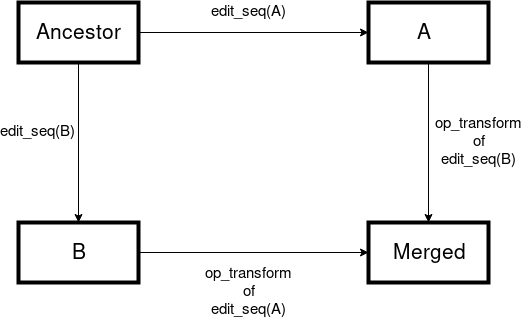
\includegraphics[width=0.7\textwidth]{merge-square.png}
\end{figure}

We can define the Edit sequence operations using the Abstraction operations, independent from the implementation. 
\begin{table}[h]
\centering
\begin{tabular*}{\columnwidth}{@{\extracolsep{\stretch{1}}}*{7}{ll}@{}}
\hline
\textbf{Abstraction} & \textbf{Edit Sequence Structures} \\ \hline
Vector & \begin{tabular}[c]{@{}l@{}}Insert (i, E)\\ Replace (i, A, E) \\ Remove(i)\end{tabular} \\ \hline
Set & \begin{tabular}[c]{@{}l@{}}Add (E)\\ Remove(E)\end{tabular} \\ \hline
Map & \begin{tabular}[c]{@{}l@{}}Add(K, E)\\ Remove(K)\\ Replace(K, A, E)\end{tabular} \\ \hline
Heap & \begin{tabular}[c]{@{}l@{}}Delete-Min (E)\\ Insert (E)\end{tabular} \\ \hline
\end{tabular*}
\end{table}

\lstinline{op_transform} takes a pair of edit sequences \lstinline{s1} and \lstinline{s2}, that map a structure \lstinline{v} to two different structures \lstinline{v1} and \lstinline{v2}, and transforms \lstinline{s1} to \lstinline{s1'} such that \lstinline{s1'} has the same effect on \lstinline{v2} as \lstinline{s1} had on \lstinline{v} \cite{mergeable-types}.

\newpage
\section{Vector}
\subsection{Vector signature}
\begin{lstlisting}
module type Base = sig
  type atom
  type t
  val length : t -> int
  val set : t -> int -> atom -> t
  val get : t -> int -> atom
  val insert : t -> int -> atom -> t
  val delete : t -> int -> t
end
\end{lstlisting}

\subsection{Vector - List implementation}
\subsubsection{Basic operations}
Simple Vector implementation using the Lists from Ocaml stdlib. All Vector operations can be performed with O(n) time complexity.
\subsubsection{Edit sequence generation}
The algorithm uses O($n^{2}$) time string edit distance algorithm described in \cite{wagner-fischer-1974} and \cite{mergeable-types} that has O(mn) time complexity. 
\subsubsection{Operational transform}
Given edit sequences as in \ref{mtype-framework}: 
\begin{itemize}
\item Order of the elements is retained. 
\item Non conflicting substitution at a position is a substitution operation in s1'.
\item Substitution conflict with a deletion is a no-op in s1', so that deletion wins for the final merged vector. 
\item Substitution conflict with another substitution is handled by a user defined merge of the atomic value in s1'. 
\end{itemize}

The operational transform algorithm has a complexity of O(m + n) where m, n are lengths of the edit sequences.

\newpage
\section{Set}
\subsection{Set signature}
This is a simplified Set signature. The implementation is compatible with the full Ocaml standard library Set signature.
\begin{lstlisting}
module type Base = sig
  type t
  type atom
  val empty: t
  val is_empty: t -> bool
  val mem: atom -> t -> bool
  val add: atom -> t -> t
  val remove: atom -> t -> t
end
\end{lstlisting}

\subsection{Set - AVL tree implementation}
Ordered Set implementation from the Ocaml standard library is reused. The AVL tree has a height balancing factor of 2. All basic operations have O(log n) time complexity.
\subsubsection{Edit sequence generation}\label{set-avlt-diff}
This algorithm is an adaptation of Tarjan etal. Fast BST Merging Algorithm \cite{}. Because we have to in-order traverse both trees the complexity of this algorithm will be O(m + n)

An optimization we can do to gain major performance improvements in a content addressable storage is by doing structural comparison of the child trees before recursion. Basically if s1.hash == s2.hash, then the edit sequence is empty. This is an optimization that cannot be performed if another solution that used flattens the tree structure was used.

\begin{lstlisting}
diff t1 t2:
  # Base cases:
     Empty tree vs Some tree -> 
     	fold tree in-order 
     	  mark all as Add operations
     Some tree vs Empty tree ->
     	fold tree in-order 
     	  mark all as Remove operations
  # Recursive case:
     xx, r, yy = split the larger tree by root
     x,exists,y = split the smaller tree by r
     smaller = diff x x
  	 larger = diff y y
     if exists: 
     	smaller + larger
     else:
     	if t1 is larger tree then 
        	edit_op = Remove r
            smaller + [edit_op] + larger
        else 
        	edit_op = Add r
        	smaller + [edit_op] + larger
        
\end{lstlisting}

\subsubsection{Usage and edit sequence}
\begin{lstlisting}
let module IntAtom = struct
  type t = int
  let compare = Pervasives.compare
  let to_string = string_of_int
end in

let module M =  Mset_avltree.Make(IntAtom) in

let original = M.empty |> M.add 10 |> M.add 5 |> M.add 20 in
let v1 = original |> M.add 40 |> M.add 60 |> M.remove 10 in
let v2 = original |> M.add 4 |> M.add 3 |> M.add 2 |> M.add 1 in
let _ = M.merge3 ~ancestor:original v1 v2
;;

M.op_diff	original v1;;
- : M.edit list = [M.Remove 10; M.Add 40; M.Add 60]
M.op_diff original v2;;
- : M.edit list = [M.Add 1; M.Add 2; M.Add 3; M.Add 4]
\end{lstlisting}

\subsection{Operational transform}
Given A ancestor set, X version and Y version set: merged set will be A + X + Y - (A - X) - (A - Y).
To achieve this merged set, given edit sequences according to \ref{mtype-framework}: 
All Set Inserts and Removes performed by s1 can be directly applied on v2, and hence be included in s1'. In operational transformation we can identify few cases that can be optimized to so that s1' sequence is shorter.
\begin{itemize}
\item Inserts of equal values in both sequences, is a no-op in s1'
\item. Removes of equal values in both sequences is a no-op in s1'
\item Insert and Remove of equal values is not possible because of Set's uniqueness property.
\end{itemize}
\subsection{Example}
\begin{figure}[H]
  \begin{subfigure}{\linewidth}
  \begin{center}
  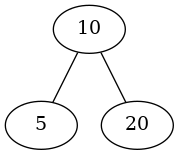
\includegraphics[height=.2\textheight,keepaspectratio]{set-avl-original.png}
  \end{center}
  \caption{Original tree}
  \end{subfigure}\par\medskip
  \begin{subfigure}{\linewidth}
  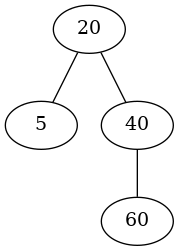
\includegraphics[width=.3\linewidth, height=.3\textheight,keepaspectratio]{set-avl-v1.png}\hfill
  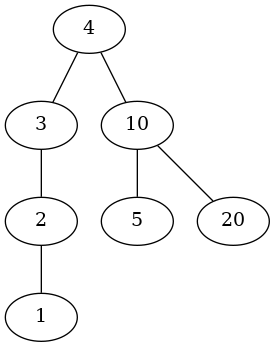
\includegraphics[width=.4\linewidth,height=.4\textheight,keepaspectratio]{set-avl-v2.png}
  \caption{v1 and v2 on left and right respectively}
  \end{subfigure}\par\medskip
  \begin{subfigure}{\linewidth}
  \begin{center}
  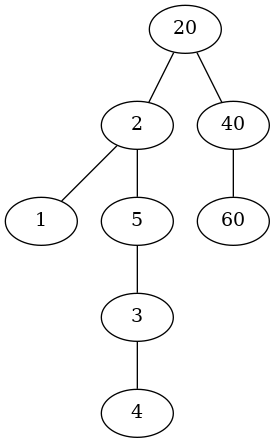
\includegraphics[height=.3\textheight,keepaspectratio]{set-avl-merged.png}
  \end{center}
  \caption{Merged AVL trees}
  \end{subfigure}
\end{figure}

\newpage
\section{Map}
\subsection{Map signature}
\begin{lstlisting}
module type Base = sig
  type t
  type key
  type atom
  val empty : unit -> t
  val is_empty : t -> bool
  val mem : key -> t -> bool
  val add : key -> atom -> t -> t
  val remove : key -> t -> t
  val compare : (atom -> atom -> int) -> t -> t -> int
  val equal : t -> t -> bool
  val iter : (key -> atom -> unit) -> t -> unit
  val fold : (key -> atom -> atom -> atom) -> t -> atom -> atom
  val find : key -> t -> atom
  val map : (atom -> atom) -> t -> t
  val mapi : (key -> atom -> atom) -> t -> t
end
\end{lstlisting}

\subsection{Map - AVL tree implementation}
Ordered map implementation from the Ocaml stdlib is reused. The AVL tree has a height balancing factor of 2. All operations have O(log n) time complexity.

\subsubsection{Edit sequence generation}
This algorithm is similar to the previously discussed algorithm in \ref{set-avlt-diff}. Differences lies on the markings to support Key conflicts.

\begin{lstlisting}
diff t1 t2:
  # Base cases:
     Empty tree vs Some tree -> 
     	fold tree in-order 
     	  mark all as Add (key, value) operations
     Some tree vs Empty tree ->
     	fold tree in-order 
     	  mark all as Remove (key) operations
  # Recursive case:
     xx, key, yy = split the larger tree by root
     x,exists,y = split the smaller tree by key
     smaller = diff x x
  	 larger = diff y y
     if exists:
     	if t1[key] == t2[key]
     		return smaller + larger
        else
        	edit_op = Replace (key, t1[key], t2[key])
            return smaller + [edit_op] + larger
     else:
     	if t1 is larger tree then 
        	edit_op = Remove key
            return smaller + [edit_op] + larger
        else 
        	edit_op = Add (key, value)
        	return smaller + [edit_op] + larger
\end{lstlisting}

\subsubsection{Usage and edit sequence}
\begin{lstlisting}
let module IntAtom = struct
  type t = int
  let resolve x y = x + y
  let merge3 ~ancestor x y = ancestor + (x - ancestor) + (y - ancestor)
  let to_string = string_of_int
  let equal x y = Pervasives.compare x y = 0 
end in

let module StringKey = struct
  include String
  let to_string s = s 
end in

let module M = Mmap_avltree.Make(StringKey)(IntAtom) in
let original = M.empty () |> M.add "C" 10 
               |> M.add "A" 5 |> M.add "D" 20 in
let v1 = original |> M.add "A" 40 
         |> M.add "D" 60 |> M.remove "C" in
let v2 = original |> M.add "Z" 4 
         |> M.add "D" 70 in
let _ = M.merge3 ~ancestor:original v1 v2
;;
M.op_diff	original v1;;

M.op_diff original v2;;

\end{lstlisting}


\subsection{Map - Trie implementation}
Trie is implemented as a Map of mergeable Maps, where the key of a trie is a list of keys of the map. Basic operations have a O(k log n) worst case time complexity (k = length of the key list), and n is the size of largest map. Since the search space of conflicting keys per map is smaller the complexity of merge operations is much smaller than an implementation without tries.

\subsubsection{Merge operation}
By using the compositionality of Maps, we can define the Trie merge operation, without using edit sequences.

\subsubsection{Usage}
\begin{lstlisting}
let module IntAtom = struct
  type t = int
  let resolve x y = x + y
  let merge3 ~ancestor x y = ancestor + (x - ancestor) + (y - ancestor)
  let to_string = string_of_int
  let equal x y = Pervasives.compare x y = 0 
end in

let module StringKey = struct
  include String
  let to_string s = s 
end in

let module M = Mmap_trie.Make(StringKey)(IntAtom) in
let original = M.empty () |> M.add ["C"] 10 |> M.add ["C"; "A"] 5 |> M.add ["D"] 20 in
let v1 = original |> M.add ["C"; "A"] 40 |> M.add ["C"; "A"; "R"] 60 |> M.remove ["C"] in
let v2 = original |> M.add ["Z"] 4 |> M.add ["D"] 70 in
let _ = M.merge3 ~ancestor:original v1 v2
;;;
\end{lstlisting}

\subsection{Operational transform}
Given edit sequences as in \ref{mtype-framework}: 
All non-conflicting Key Inserts and Removes can be performed directly on v2 and hence be included in s1'. In operational transformation we can identify the following cases:
\begin{itemize}
\item Inserts of equal Keys(k) in both sequences, is a Replace(k, User defined merge for the two atomic values) in s1'
\item Removal of equal keys, is a no-op in s1'
\item Insert and remove of equal values is not possible because of Key uniqueness
\item Replace of equal Keys(k) in both sequences, is a Replace(k, User defined merge for the two atomic values) in s1'
\end{itemize}
This algorithm has O(m + n) complexity assuming that the Edit operations of each version is sorted by their Keys.
\subsection{Example}
\mytodo{includegraphics Map - AVL tree merge}

\newpage
\section{Heap}
\subsection{Heap signature}
\begin{lstlisting}
module type Base = sig
  type t
  type atom

  val empty : t
  val is_empty : t -> bool
  val insert : atom -> t -> t
  val merge : t -> t -> t
  val find_min : t -> atom 
  val delete_min : t -> atom * t
end
\end{lstlisting}

\subsection{Heap - Leftist heap implementation}
Leftist heap implementation as described in Purely Functional Data structures\cite{okasaki}. Insert, merge and delete-min operations have a O(log n) time complexity, and Find-min operation has O(1) time complexity.

\subsection{Heap - Binomial heap implementation}
Binomial heap implementation as described in Purely Functional Data structures\cite{okasaki}. Insert, merge, find-min and delete-min operations have a O(log n) worst case time complexity, but Insert has a O(1) amortized time complexity.

\subsection{Heap - Pairing heap implementation}
Pairing heap implementation as described in Purely Functional Data structures\cite{okasaki}. Insert and Merge has O(1) time complexity and Merge and Delete-min has O(log n) amortized time complexity.

\subsection{Edit sequence generation}
Simple Edit sequence generation is comparing the minimum (or maximum) of the heaps until either heap is empty. All heap implementations share the same algorithm, time complexity will be dependent upon the time complexity of Delete-min operation. If we take delete-min has a O(g(n)) time complexity then the Edit sequence generation algorithm will have a O(n g(n) + m g(m)) time complexity.
\begin{lstlisting}
diff hx hy =
  # Base case:
  	Both heaps are empty -> return []
  # Recursive cases:
  	if hx is empty:
      m, hy = delete_root hy in
      Insert m :: diff hx hy
  	else if hy is empty:
      let m, hx = delete_root hx in
      Delete m :: diff hx hy
  	else:
      compare heap roots
      if roots are equal
      	hx, hy = remove root of both heaps
        diff hx hy
      else
      	hx, hy = remove root of heap with smaller root
        [edit op] :: diff hx hy
\end{lstlisting}

\subsection{Operation transform}
Because Heaps allow duplicate values, conflicting operations leads to implementation choices.
\begin{itemize}
\item Inserts of equal values, either no-op or another Insert in s1'. Depending on the choice the merged heap will have either single Insert or Two Inserts. Current implementation chooses Two inserts.
\item Delete of equal keys must be a no-op in s1'
\item Delete and Insert of equal keys is a choice in allowing Inserts or Deletes to take precedence.
\end{itemize}
This algorithm has a O(m+n) time complexity given that the values are in sorted order, which we ensure in edit sequence generation.
\subsection{Example}
\mytodo{includegraphics Heap merge diagrams}

\newpage
\section{Usage examples}
\subsection{Key value store of string documents}
Modeled using a Trie Map of mergeable vectors
\begin{lstlisting}
module RString = struct
  module A = struct
    type t = char
    let resolve x y = 'f'
    let merge3 ~ancestor x y = 'f'
  end
  module V = struct
    type atom = char
    type t = string
    .. removed for clarity ..
  end
  module M = Mvector.Make(A)(V)
  include M
  let equal (x:M.t) (y:M.t) = String.equal x y
  let resolve (x:M.t) (y:M.t):M.t = .. removed for clarity ..
end

module V = Mvector_list.Make(RString)

module IntKey = struct
  type t = int 
  let compare = compare
  let to_string = string_of_int
end
module M = Mmap_trie.Make(IntKey)(RString)(Mmap_avltree.Make)

let kls x = 
  List.fold_left (fun x y -> x ^ IntKey.to_string y) "" x

let _ =
  let original = M.empty () |> M.add [1] "ehllo" |> 
                 M.add [1;2] "hello world" in
  let v1 = original |> M.add [1] "hello" 
           |> M.add [1; 2] "hello there" in
  let v2 = original |> M.add [1] "hello" 
           |> M.add [1; 2] "hello ocaml" |> M.add [2] "bye" in
  let m = M.merge3 ~ancestor:original v1 v2 in
  M.iter (fun k s -> Printf.printf "%s\n" ((kls k)^":"^s)) m
\end{lstlisting}

\newpage
\section{Single node performance}
To examine the overhead of lineage tracking and using the merge framework:
\begin{figure}[h]
\centering
\caption{Single process handling all operations from a producer}
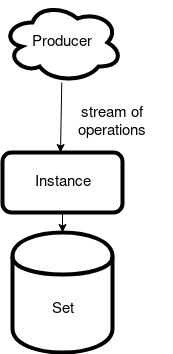
\includegraphics[width=0.2\textheight]{benchmark-single.png}
\end{figure}
\begin{figure}[h]
\centering
\caption{Multiple processes handling operations from a producer, using locks to handle the shared data structure}
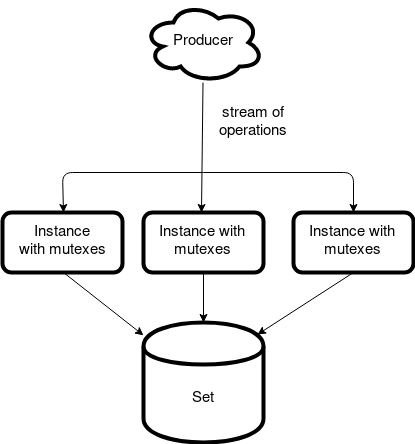
\includegraphics[width=0.3\textheight]{benchmark-mutexes.png}
\end{figure}
\begin{figure}[h]
\centering
\caption{Multiple processes handling operations from a producer, using mergeaable types storage to handle the shared data structure}
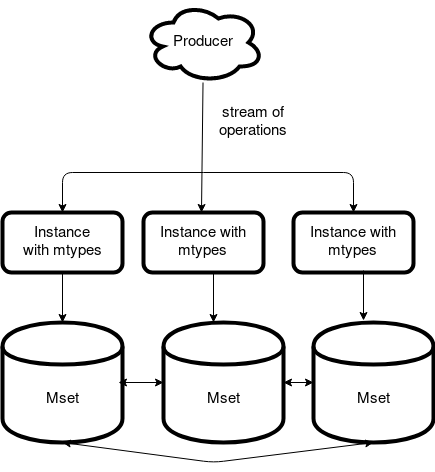
\includegraphics[width=0.3\textheight]{benchmark-mtyped.png}
\end{figure}
\end{document}